\section{Reputation Mining}\label{sec:reputationmining}

The reputation system is a core component of any decentralised colony. By carefully balancing the rewards and penalties we aim to keep every users' incentives aligned with the colony and the colony network. Since reputation can only be \emph{earned} and not transferred between accounts, the system fosters a more meritocratic form of decision making than pure token-weighted voting can hope to achieve. The continuous decay of reputation ensures that the influence conveyed by reputation is recently earned and up-to-date. As such, it prevents a reputation aristocracy and allows for a fluid passing of control from one set of contributors to another over time.


Due to the combined complexity of reputation scores across multiple colonies, domains, and skills, reputation scores cannot be stored or calculated on-chain. Instead, the calculations will all take place off-chain, the results of which will be reported to the blockchain by participating CLNY holders --- in a process resembling a proof-of-stake blockchain consensus protocol. We call this procedure \textbf{Reputation Mining}.

The reputation calculation whose result the miners are submitting is determined by the activities that have taken place in the colonies and can be fully deterministically derived from the Ethereum blockchain. Game-theoretically the system is protected similarly to the off-chain calculations of TrueBit (\cite{TruebitWhitepaper}) in that, \emph{while the calculation cannot be done on-chain and a correct submission can never be proved true, an incorrect calculation can always be proved to be wrong}.


\subsection{Merkle-Patricia trees and proofs}\label{sec:Merkle-summary}
This subsection contains only a summary of Merkle-Patricia trees (\cite{MerkleTrees}, \cite{MerkleInEthereum}) and Merkle proofs in order to establish some terminology, and can be skipped if already familiar with them.

A Merkle-Patricia tree, or `trie', is a key-value store with two special properties: efficient insertion and lookup, and a compact cryptographic state signature. Put succinctly, it is Patricia in the branches, and Merkle in the nodes -- the branching of the tree is determined by the keys (in a way which avoids redundant tree traversal), while the values in the nodes are determined by recursively hashing the values inserted in the leaves.

Consider the tree shown in Figure \ref{fig:Merkleexample}, in which every values has a 4-bit key. The data leaves of the tree (1, 2, 3 and 4), which correspond to the keys (0000, 0010, 00111, and 1011), are each hashed individually to give A, B, C and D. These are then repeatedly hashed pairwise, following the branching structure determined by the keys, until only a single hash remains, indicated by G. The resulting structure is known as a Merkle-Patricia tree. In order to prove that the element \ascode{1} is in the tree with root \ascode{G}, one submits a Merkle proof containing the information \ascode{(0000, 1, [E,D], [1010])}. The first pair of arguments are the key-value pair whose existence is to be proved. The third argument is the array of node hashes (`siblings') that the leaf hash should be recursively hashed with. The last argument, the `branch mask', is an array of \ascode{1}'s and \ascode{0}'s that indicate which bits of they key correspond to the branching points (in this case, the first and third most-significant bits). So to show that \ascode{3} was in the tree with root \ascode{G}, the proof would be of the form \ascode{(0011, 3, [B,A,D], [1011])}.

\begin{figure}
\centering
 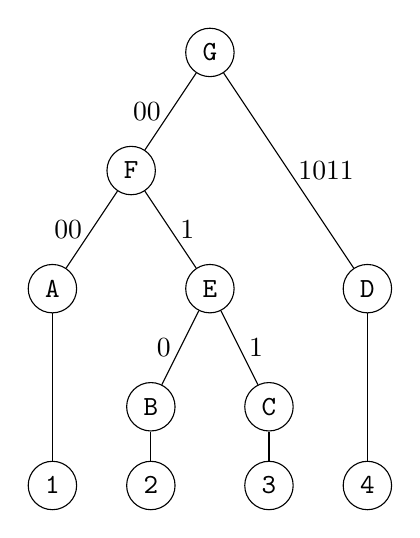
\begin{tikzpicture}
  \node[shape=circle, draw] at (-0.5,-3) (a) {\texttt{A}};
  \node[shape=circle, draw] at (-0.5,-5.5) (1) {\texttt{1}}
   edge[-] (a);

  \node[shape=circle, draw] at (.75,-4.5) (b) {\texttt{B}};
  \node[shape=circle, draw] at (.75,-5.5) (2) {\texttt{2}}
   edge[-] (b);

  \node[shape=circle, draw] at (2.25,-4.5) (c) {\texttt{C}};
  \node[shape=circle, draw] at (2.25,-5.5) (3) {\texttt{3}}
   edge[-] (c);

  \node[shape=circle, draw] at (3.5,-3) (d) {\texttt{D}};
  \node[shape=circle, draw] at (3.5,-5.5) (4) {\texttt{4}}
   edge[-] (d);

  \node[shape=circle, draw] at (1.5,-3) (e) {\texttt{E}}
   edge[-] node[left] {0} (b)
   edge[-] node[right] {1} (c);

  \node[shape=circle, draw] at (.5,-1.5) (f) {\texttt{F}}
   edge[-] node[left] {00} (a)
   edge[-] node[right] {1} (e);

  \node[shape=circle, draw] at (1.5,0) (g) {\texttt{G}}
   edge[-] node[left] {00} (f)
   edge[-] node[right] {1011} (d);
 \end{tikzpicture}
 \caption{A simple Merkle-Patricia tree with 4-bit keys. Element A is the hash of value 1, with a key of 0000. Element E is the hash of B concatenated with C, and so on recursively up to the root G. Changing any leaf value will change the root, the essential property.}
 \label{fig:Merkleexample}
\end{figure}


\subsection{The Reputation Tree}\label{sec:reptree}

The key-value pairs in the reputation tree are the reputations all users have in all skills, as well as the colony-wide totals. A single key-value pair consists of the following data:
\begin{align*}
k &=
  \begin{cases}
  \ascode{colony} & \textnormal{address of the colony the reputation is in}\\
  \ascode{user} & \textnormal{account address holding the reputation}\\
  \ascode{skill} & \textnormal{skill id of the reputation}
  \end{cases}\\
v &=
  \begin{cases}
  \ascode{amount} & \textnormal{numerical value of the reputation}\\
  \ascode{nonce} & \textnormal{unique per-leaf id (used in reputation mining)}
  \end{cases}
\end{align*}

All individual reputations are assembled into the \textbf{Reputation Tree} which is a Merkle-Patricia tree of all individual reputations in a colony, as well as the total reputation of each type held by the users in each colony. The leaves that represent these colony-wide totals are indicated by setting \ascode{user} to zero. These leaves are then inserted into the tree as described in Section \ref{sec:Merkle-summary}. We term the root hash of the resulting tree the \ascode{ReputationRootHash}, $\mathcal{RH}$.
\begin{figure}
\centering
\begin{tikzpicture}
 \node at (0,-5) (r0) {$R_0$};
 \node at (1.5,-5) (r1) {$R_1$};
 \node at (3,-5) (r2) {$R_2$};
 \node at (4.5,-5) (r3) {$R_3$};
 \node at (6,-5) (rdots) {$\cdots$};
 \node at (8,-5) (rn) {$R_N$};
 %
 \node at (0,-4) (r0hash) {$\mathcal{H}(R_0)$}
  edge[-] (r0);
 \node at (1.5,-4) (r1hash) {$\mathcal{H}(R_1)$}
  edge[-] (r1);
 \node at (3,-4) (r2hash) {$\mathcal{H}(R_2)$}
  edge[-] (r2);
 \node at (4.5,-4) (r3hash) {$\mathcal{H}(R_3)$}
  edge[-] (r3);
 \node at (8,-4) (rnhash) {$\mathcal{H}(R_N)$}
  edge[-] (rn);
 %
 \node at (0.75,-2.5) (r01) {$\mathcal{H}_{0,1}$}
  edge[-] (r0hash)
  edge[-] (r1hash);
 \node at (3.75,-2.5) (r23) {$\mathcal{H}_{2,3}$}
  edge[-] (r2hash)
  edge[-] (r3hash);
 \node at (7,-2.5) (rnn) {$\mathcal{H}_{N-1,N}$}
  edge[-] (rnhash)
  edge[dashed] (6.5,-4);
 %
 \node at (2.25,-1) (r14) {$\mathcal{H}_{0,3}$}
  edge[-] (r01)
  edge[-] (r23);
 %
 \node[draw, fill=gray!5] at (4,0) (root) {\texttt{ReputationRootHash}  ($\mathcal{RH}$)};
 \node[below = 1mm of root] (dummy) {\phantom{a}}
  (dummy.north west) edge[dashed] (r14)
  (dummy.north east) edge[dashed] (rnn);
 %
 %
\end{tikzpicture}
\caption{The Merkle tree of users' reputations with \ascode{ReputationRootHash} as the root. We use $\mathcal{H}$ to indicate the \ascode{keccak256} hash function.}
\end{figure}


The \ascode{ReputationRootHash} is the only data we record on the blockchain associated with users' reputations. It summarises the state of the whole reputation system and whenever a user wishes to make use of their reputation, they can submit a Merkle proof from the reputation $\mathcal{R}_i$ they wish to make use of and ending at $\mathcal{RH}$.

\subsection{Calculating the new root hash}
To calculate the new root hash, the miners begin with the last reputation state, and decay all reputations held by all users in all colonies, in the order of the leaf nonces. They then take the set of reputation gains or losses that were not in the last state submitted, and are to be included in the next state (the update log). They apply the reputation updates to each user in each colony, updating or adding leaves as necessary (following the process described in \ref{sec:justificationTree}), to end up with a new list of reputations for all users and colonies. These new reputations are then hashed and assembled into a new Merkle-Patricia tree yielding an updated \ascode{ReputationRootHash}.

While the calculation is too large to be done on-chain due to technical and economic limitations (i.e. the block gas limit and the cost of gas, respectively), this calculation can easily be performed by a typical user's computer.

\subsection{Submission of a new root hash}
%
\subsubsection*{What is submitted?}
The final \ascode{ReputationRootHash} is submitted to the contract by the miner along with the number of leaves in the tree (\ascode{NReputationLeaves}). The miner also submits the root hash of the Justification Tree (see Section \ref{sec:justificationTree}), which will be used in the event of a dispute. These three properties uniquely identify a submission.
%
\subsubsection*{Who can submit a new root hash?}
All \rcths\ are eligible to become miners and participate in the reputation update process. Since any user can calculate the correct root hash locally, it should be possible for \emph{any} miner to submit the hash to the contract.

It is however undesirable to have too many submissions for every update. We propose a mechanism that only allows some miners to submit results to begin with. To participate in the mining process, \rcths\ must stake some of their tokens to become `reputation miners'. A submission will only be accepted from a miner if
\begin{equation*}\label{eq:mining-difficulty}
\ascode{uint256(keccak256(address, N, hash))} < \ascode{target}.\footnote{Note that internally the arguments are encoded using \ascode{abi.encodePacked} before being hashed.}
\end{equation*}
At the beginning of the submission window, the target is set to 0 and slowly increases to $2^{256}-1$ after \miningcycleduration\ hour. We limit the total number of miners allowed to submit a specific hash to 12. In the unlikely event that no submissions are received before the \miningcycleduration-hour window has elapsed, exactly one submission will be accepted, whenever it is received.

The variable $N$ that goes into the hash is some integer greater than 0 and less than the number of tokens the \rcth\ account has staked divided by \minstake\, meaning that users with a large stake have a higher chance of qualifying to submit a hash sooner than smaller stake holders. The factor of \minstake\ is introduced to ensure that all hashes a user is eligible to submit can be calculated in a few seconds by the client. It also effectively creates a minimum number of tokens that must be staked to submit a hash. This puts a tangible cost on any attacks revolving around spamming known false submissions (see Section \ref{sec:mining-possible-attacks}).

When a miner stakes, the timestamp of the stake is recorded.\footnote{If a miner adds additional stake, the timestamp is set to the weighted average of the existing and new timestamps.} In order to be eligible to submit a hash, the miner must have staked before the beginning of the current mining cycle.

\subsubsection*{Verifying a submission}
If only one state is submitted by the end of the submission period, then the new state is accepted, and proposals of the next state can begin to be made. This is expected to be the most common occurrence.

If more than one state has been submitted, then either someone has made a mistake, or there is a malicious entity trying to introduce a fraudulent reputation change. In this event, the challenge-response protocol can establish which state is incorrect (see Section \ref{sec:challenge-response}).

\subsubsection*{Mining rewards}

When a state is accepted, a number of (newly minted) \rcts\ are made available for the users who submitted the correct state to claim as a reward. They also receive a corresponding amount of reputation in the \rc\ (in a special mining skill, which only users in the \rc\ can earn by performing this task). This reputation update is no different from any other, aside from the limitations of who is able to earn it, and will be included in the subsequent reputation update cycle. The size of the rewards and their distribution are described in Section \ref{subsec:mining-costs-and-rewards}.

\subsection{Dealing with false submissions}\label{sec:challenge-response}

We assume that the correct hash is one of the  submitted hashes. This is a reasonable assumption, as only one out of all the miners is required to make a correct submission, and there is an incentive for them to do so (the reward defined in Section \ref{subsec:mining-costs-and-rewards}). Thus our task is not to validate the correct hash but to invalidate the false one(s).

We must prove all but one submission incorrect by having each submission prove that they calculated more correct reputation updates before getting one wrong (if any) than another submission they are being compared against. Anyone is able to respond to a challenge (and be rewarded), regardless of who submitted the original hash; this should ensure that the correct state is always defended, even if some miners go offline.

We consider the scenario where only two submissions are made, and one is correct. In the event of more than two submissions, this same pair-wise comparison described below is repeatedly run (in parallel, where possible) among remaining submissions until only one remains.

\subsubsection{The Justification Tree}\label{sec:justificationTree}
\newcommand{\jrh}{\ensuremath{\mathbb{JRH}}}

A client submits a \ascode{JustificationRootHash} (\jrh) as part of the process of submitting a proposed new root hash. This is the Merkle root of the `Justification Tree' -- a Merkle-Patricia tree where each leaf represents not a single reputation value, but the root hash of an entire reputation state. The left-most leaf of the Justification Tree is the final accepted reputation state from the last update ($\mathcal{RH}_0$) concatenated with the number of leaves ($\mathcal{L}_0$) in the reputation tree $\mathcal{RH}_0$ is the root of. The right-most leaf of the Justification Tree is the \ascode{ReputationRootHash} they submitted ($\mathcal{RH}_N$) concatenated with the number of leaves it contains ($\mathcal{L}_N$). We denote these leaves as $\mathcal{RH}_0 \cdot \mathcal{L}_0$ and $\mathcal{RH}_N \cdot \mathcal{L}_N$.

The intermediate leaves represent the evolution of the global reputation state after applying some subset of the full sequence of reputation updates required. Each state represented by a leaf differs from the reputation states in neighboring leaves in \textit{at most} a single reputation.\footnote{It is possible for two adjacent leaves to be identical if the reputation update the transition between them represents does not result in a change in reputation -- e.g. a reputation loss in a reputation that is already zero.} In order to do this in a consistent way, we must order all the updates in a reputation cycle. The canonical ordering for reputation updates is:

\begin{enumerate}
\item All decays of existing reputations, in order of \ascode{nonce},
\item The entries in the reputation update log, in order of appearance in the reputation update log. A single one of these entries corresponds to at least two reputation updates with an unbounded upper limit (since there can be many parent and child updates). These updates are themselves ordered:
\begin{enumerate}
  \item Colony-wide total of any impacted child reputations \label{lab:colonyWideChildren}
  \item Colony-wide total of any impacted parent reputations \label{lab:colonyWideParents}
  \item The colony-wide total of the origin reputation
  \item User-specific child reputations \label{lab:userChildren}
  \item User-specific parent reputations\label{lab:userParents}
  \item User-specific origin reputation
\end{enumerate}
The origin reputation is defined to be the skill specified in the reputation log where the reputation is to be lost or gained. Where multiple child reputations are required to be updated as part of \ref{lab:colonyWideChildren} or \ref{lab:userChildren}, they are done so in the order they appear in the \ascode{children} property of the origin skill. Where multiple parent reputations are required to be updated as part of \ref{lab:colonyWideParents} or \ref{lab:userParents}, the immediate parent is updated first, then the immediate parent of that skill, and so on until no parents remain. We do the decay calculations first to give users the benefit of the doubt during reputation updates so they do not lose reputation they have only just earned to premature decay.
\end{enumerate}

As a miner applies the reputation updates for a cycle in this order, they should take each intermediate \ascode{ReputationRootHash} values and build the Justification Tree by adding the intermediate \ascode{ReputationRootHash} values concatenated with \ascode{NReputationLeaves} to the tree, \textit{with key equal to the update number}, starting from 0. Note that unlike in the Reputation Tree, the keys should not be hashed. This will become important further on in the dispute process, as we will need to be able to identify sequentially adjacent reputation updates. The intermediate leaves of the Justification Tree represent the evolution of the reputation state, with $\mathcal{RH}_i$ corresponding to the reputation state after the first $i$ reputation updates in this cycle have been applied. An example of such a tree is shown in Figure \ref{fig:justification-tree}.

 %
\begin{figure}
\centering

\begin{tikzpicture}
 \node at (0,-5) (r0) {$RH_0\cdot \mathcal{L}_0$};
 \node at (2.5,-5) (r1) {$RH_1\cdot \mathcal{L}_1$};
 \node at (5,-5) (r2) {$RH_2\cdot \mathcal{L}_2$};
 \node at (7.5,-5) (r3) {$RH_3\cdot \mathcal{L}_3$};
 \node at (9,-5) (rdots) {$\cdots$};
 \node at (11,-5) (rn) {$RH_N\cdot \mathcal{L}_N$};
 %
 \node at (0,-4) (r0hash) {$\mathcal{H}(RH_0\cdot \mathcal{L}_0)$}
  edge[-] (r0);
 \node at (2.5,-4) (r1hash) {$\mathcal{H}(RH_1\cdot \mathcal{L}_1)$}
  edge[-] (r1);
 \node at (5,-4) (r2hash) {$\mathcal{H}(RH_2\cdot \mathcal{L}_2)$}
  edge[-] (r2);
 \node at (7.5,-4) (r3hash) {$\mathcal{H}(RH_3\cdot \mathcal{L}_3)$}
  edge[-] (r3);
 \node at (11,-4) (rnhash) {$\mathcal{H}(RH_N\cdot \mathcal{L}_N)$}
  edge[-] (rn);
 %
 \node at (1.25,-2.5) (r01) {}
  edge[-] node[left=1mm] {0} (r0hash)
  edge[-] node[right=1mm] {1} (r1hash);
 \node at (6.25,-2.5) (r23) {}
  edge[-] node[left=1mm] {0} (r2hash)
  edge[-] node[right=1mm] {1} (r3hash);
 \node at (10,-2.5) (rnn) {}
  edge[-] (rnhash)
  edge[dashed] (9,-4);
 %
 \node at (3.75,-1) (r14) {}
  edge[-] node[left=2.5mm] {0} (r01)
  edge[-] node[right=2.5mm] {1} (r23);
 %
 \node[draw, fill=gray!5] at (6.5,0) (root) {\texttt{Justification Root Hash}  (\jrh)};
 \node[below = 1mm of root] (dummy) {\phantom{a}}
  (dummy.north west) edge[dashed] (r14)
  (dummy.north east) edge[dashed] (rnn);
 %
 %
\end{tikzpicture}
\caption{The Justification Tree. The leaf containing $\mathcal{H}(RH_0\cdot \mathcal{L}_0)$ -- the last accepted reputation state -- is found at key \ascode{...00}. The leaf containing $\mathcal{H}(RH_1\cdot \mathcal{L}_1)$ -- the reputation state with the decay of the existing skill with nonce 0 applied -- is found at key \ascode{...01}. Every intermediate state is recorded in the tree up to $\mathcal{H}(RH_N\cdot \mathcal{L}_N)$, which is the proposed new reputation state with all reputation updates applied.}
\label{fig:justification-tree}
\end{figure}

\subsubsection{Resolving a dispute}

If a dispute occurs, the first step is for each submission to verify the Justification Tree they submitted alongside their proposed new root hash.

\subsubsection*{1. Verifying the Justification Tree}

For a justification tree to be deemed valid, it must:

\begin{itemize}
\item Have $\mathcal{H}(RH_0 \cdot \mathcal{L}_0)$ at key 0,
\item Have $\mathcal{H}(RH_N \cdot \mathcal{L}_N)$ at key $N$,
\item Have a plausible structure.
\end{itemize}

The first two items are relatively straightforward to prove via Merkle proof. The last requirement requires slightly more explanation. A Justification Tree with two leaves could meet the first two requirements, but we would be able to tell this tree wasn't plausible as a Justification Tree because the Merkle proofs supplied to prove the first two requirements would not be of the expected length.\footnote{We know that every reputation cycle will at least have log entries for rewarding those who submitted the previous reputation state successfully.} This length is calculable because we know how many leaves are meant to be in the tree and what keys they are expected to be at (every key between 0 and $N$). We are also able to determine the branchmasks that these proofs should have (the binary representations of $2^{\lceil\log_2 (N+1) \rceil} - 1$, and $N$ respectively), which further constrains the shape of a plausible tree.

Unfortunately, based on these two proofs, we are unable to guarantee the Justification Tree contains a leaf at every key from 0 to $N$. This is because we do not know how many leaves the siblings used in the Merkle proofs contain, and it is not feasible to request a proof for every key between $1$ and $N-1$. This is why the constraint is limited to being `plausible'. With the approach we have taken, however, we are at least able to guarantee that key $N$ is the last in the Justification Tree, that key $0$ is the first (though this is a trivial consequence of it existing), and there are at least some number of other keys in the tree.\footnote{This number is $\lceil\log_2 (N+1) \rceil + \#_{1}(N) - 2$, where $\#_{1}(N)$ is the binary logarithm of the $N$th integer in Gould's sequence. To derive this expression, consider how many siblings each proof requires; each sibling corresponds to at least one other key. In our case, $\#_{1}(N)$ provides the number of set bits in the branchmask of the proof for key $N$ i.e. how many siblings that the Merkle proof of key $N$ has. The $-2$ accounts for the key-value pairs stored at 0 and $N$.}

Since any two differing submitted states agree on the first leaf $\mathcal{RH}_0$ (the \ascode{ReputationRootHash} accepted at the end of the previous iteration of the mining cycle), and disagree on the last leaf $\mathcal{RH}_N$ (the hash they submitted), there must be a hash $\mathcal{RH}_i$ that they agree on, and a hash that $\mathcal{RH}_{i+1}$ that they do not. This is a reputation update where they agree on the starting state but disagree on the result. This transition is meant to be the effect of a single reputation update (the $i^{th}$), and this is the reputation update we will calculate on-chain to establish which submission is incorrect.\\

\noindent First, however, we must establish where the two submissions begin to differ.

\subsubsection*{2. Searching for the discrepancy}
The contract requires both parties to submit repeated Merkle proofs to locate $\mathcal{RH}_{i+1}$, the first disagreement hash. We shall call the two parties $A$ and $B$ and we shall indicate which party made a submission by a superscript of $A$ or $B$. Furthermore we introduce the simplifying notation of $\overline{h}$ to mean `sibling of $h$' in the Merkle tree.

Along with their justification root hashes $\jrh^A$ and $\jrh^B$ both parties have already submitted proofs for the left-most leaf. Ignoring the branchmasks for simplicity, these proofs have the form:
\[
 \overline{\mathcal{RH}_0}^A, \overline{h_{0,1}}^A, \overline{h_{0,2}}^A, \ldots \overline{h_{0,2^k}}^A \qquad \textnormal{ terminating at } \jrh^A
\]
and
\[
 \overline{\mathcal{RH}_0}^B, \overline{h_{0,1}}^B, \overline{h_{0,2}}^B, \ldots \overline{h_{0,2^k}}^B \qquad \textnormal{ terminating at } \jrh^B
\]
where $k$ is the largest integer such that $2^k$ is smaller than $n$.

When the first miner (say $A$) submits their proof the contract saves the values of $h_{0,2^k}^A$ and $\overline{h_{0,2^k}}^A$. When the second miner submits their proof the contract compares $h_{0,2^k}^A$ to $h_{0,2^k}^B$. If they are not equal, the contract saves both of these values (and forgets $\overline{h_{0,2^k}}^A$). If they are equal, the contract retains the values of $\overline{h_{0,2^k}}^A$ and $\overline{h_{0,2^k}}^B$ (forgetting $h_{0,2^k}^A$).

The rationale behind this behaviour is the following: If $h_{0,2^k}^A = h_{0,2^k}^B$ then the two justification trees are equal between $\mathcal{RH}_0$ and $\mathcal{RH}_{2^{k-1}}$ and the first discrepancy must lie in the right-hand subtree whose root is $\overline{h_{0,2^k}}^A$ for miner $A$ and $\overline{h_{0,2^k}}^B$ for miner $B$. If on the other hand $h_{0,2^k}^A \neq h_{0,2^k}^B$, then the first discrepancy must lie in the left-hand subtrees given by $h_{0,2^k}^A$ and $h_{0,2^k}^B$. The situation is summarised by
\begin{eqnarray*}
 h_{0,2^k}^A \neq h_{0,2^k}^B & \Longrightarrow & \textnormal{First discrepancy occurs at some } \mathcal{RH}_i \textnormal{ with } 0 \leqslant i < 2^k\\
 h_{0,2^k}^A = h_{0,2^k}^B & \Longrightarrow & \textnormal{First discrepancy occurs at some } \mathcal{RH}_i \textnormal{ with } 2^k \leqslant i < n
\end{eqnarray*}

The contract begins its search by %pseudorandomly%\footnote{This pseudorandomness is to help mitigate an attack described in Section \ref{sec:mining-possible-attacks}.}
%picking an index $j$ from within the range the first discrepancy in known to lie in. It then
%
picking an index $j$ from within the range the first discrepancy in known to lie in (say always the smallest), and requiring both parties to provide a Merkle proof showing value of \ascode{ReputationRootHash} and \ascode{NReputationLeaves} at that key in the Justification Tree. The required target of this proof is no longer the $\jrh$ itself, but rather the retained value for $h_{0,2^k}$ or $\overline{h_{0,2^k}}$.

The process as before of comparing hashes and retaining the roots of either the left-side subtree or the right-side subtree is repeated. With each iteration, the range of possible values for the index of the first discrepancy is reduced by (on average) a factor of two and the length of the required Merkle proofs is reduced by at least one.

There are two ways this process can terminate. The first way the process terminates is when one party does not respond to a challenge in adequate time, either because they could not or chose not to. In this case the party not responding is deemed to be incorrect. The other way the process terminates is when it has reached the bottom of the tree and determined $i$, the disputed reputation update.

\subsubsection*{3. Confirming $i$ }

Once the contract has found the index $i$ such that $\mathcal{RH}^A_{i}=\mathcal{RH}^B_{i}$ but $\mathcal{RH}^A_{i+1}\neq\mathcal{RH}^B_{i+1}$, the contract then requires each party to submit the value stored at the key $i+1$ in the Justification Tree to confirm that it is there. It is possible that this was already done during the binary search, but it is not guaranteed. The value of the \ascode{ReputationRootHash} and \ascode{NReputationLeaves} at this key are stored in the contract managing the dispute resolution. Again, if one party does not respond in time, they are assumed to be incorrect.

\subsubsection*{4. Deciding which submission performed the correct calculation}

In most cases, only one of the two submissions will be able to perform the transaction corresponding to this step. There are several types of calculation and checks that might need to take place, depending on which transition the two submissions first disagree on, and the values of \ascode{ReputationRootHash} and \ascode{NReputationLeaves} they placed in their Justification Trees. All of the following must be performed on chain to verify the calculation under dispute.

\begin{itemize}
\item \textbf{Check the key} As part of the Merkle proofs submitted (see the next step), the \ascode{key} of the reputation under dispute is submitted. This is a concatenation of the colony address the reputation is in, the skill the reputation is in, and the account address holding the reputation (which is possibly the zero address if the total reputation in the colony is under dispute). Based on the value of $i$, which has already been established during the binary search, and the known canonical ordering of reputation updates, the contract is able to check these values. In the case where the update under dispute is due to a log entry (as opposed to normal decay), the index of the log entry under dispute is supplied by the user and verified on-chain, to avoid iteration over the unbounded log.
\item \textbf{Check the claimed before and after values} The values of the reputation at \ascode{key} in $\mathcal{RH}_{i}$ and $\mathcal{RH}_{i+1}$ for the submission in question are proved via Merkle proof. If it is claimed an existing reputation is being updated, then the proofs' siblings and branchmask are required to be the same to guarantee no other reputations have been changed. If a new reputation is claimed to be being added (indicated by $\mathcal{L}_{i+1} - \mathcal{L}_i = 1$), the proof for the reputation in $\mathcal{RH}_i$ is not required as the reputation should not be in the tree, but an additional check will be performed later to confirm this.
\item \textbf{Perform the calculation} This has two elements. The first is to check that the \ascode{nonce} for the reputation has not changed in the leaf if an existing leaf is being updated. If a new leaf is being added, the value of the \ascode{nonce} is checked to be one larger than the $\mathcal{L}_{i}$ that they have provided (as each \ascode{nonce} is given in sequence). The second is to check that the value of the reputation is correct. It can be a decay, or an update due to an entry in the log, the potential consequences of which are described in section \ref{sec:calculating-reputation-updates}.
\item \textbf{Additional checks} Depending on the type of update being disputed, additional checks may be required
\begin{enumerate} \item Any additional reputation values needed for the calculation are proved to be in $\mathcal{RH}_{i}$ (which both parties agree on the value of) as required via Merkle proof. The canonical ordering of reputation updates ensures that any values required for the calculation under dispute are present in $\mathcal{RH}_{i}$ and have not yet been altered by the log entry under consideration.
\item Similarly, if a new leaf is added, a Merkle proof for the reputation in $\mathcal{RH}_{i}$ with the previous \ascode{nonce} is checked to confirm the \ascode{nonce} assigned to the new node is plausible.
\item If during the calculation, the user claims that a reputation they need for a calculation does not exist in $\mathcal{RH}_{i}$, and so they will use a value of 0, they must prove it does not exist in the tree.\footnote{They do this by providing a Merkle proof for an existing reputation in $\mathcal{RH}_{i}$ whose hashed key has the longest shared prefix with the hashed key of the reputation being added. By examining the branchmask of this proof, and the (hashed) keys of the proved reputation and the reputation being claimed to not exist, the contract is able to confirm the latter does not exist in $\mathcal{RH}_{i}$. If a key with a shorter shared prefix is used, the branchmask will already contain a branch point where they diverge and this proof will fail.} % I don't feel like I've explained this very well. Perhaps it warrants a subsection somewhere?
\item If a new reputation value is being added to the tree, we also prove that the reputation that it ends up closest to in the tree exists in $\mathcal{RH}_{i}$. We are therefore able to deduce what the proof for that reputation in $\mathcal{RH}_{i+1}$ should be if only the new leaf is added. By checking this Merkle proof is valid, we ensure no other changes have been made to the reputation tree.
\end{enumerate}
\end{itemize}

It is possible that both submissions will successfully submit the transaction that validates their submissions as described here. This can happen when a new leaf is being added, and the submissions have disagreed over the \ascode{nonce} the reputation should be given. Whichever has successfully awarded the highest \ascode{nonce} is deemed the correct submission. If neither party responds to a particular stage in this process in time, both are eliminated from consideration.

If the \miningcycleduration-hour mining cycle window has not elapsed by the time only one submission remains, the next window only opens when the current window has elapsed. If the \miningcycleduration-hour window has elapsed by the time the dispute process has finished, the next submission window opens immediately.

\subsection{Calculating reputation updates}\label{sec:calculating-reputation-updates}
% TODO: I think this needs to be moved to before 'Dealing with false submissions'.

\subsubsection{Keeping track of reputation changes}

Fundamentally, there are two types of reputation update that occur:
\begin{itemize}
 \item Decay of existing reputation.
 \item Addition or removal of reputation as a reward or punishment.
\end{itemize}

When a user earns reputation in a skill or domain, they also earn reputation in all parent domains, which corresponds to $2\times\left(\ascode{n\_parents}+1\right)$ reputation updates. Alternately, when a user loses reputation, they also lose reputation in all parents and all children representing a total number of updates of $2\times\left(\ascode{n\_parents} + \ascode{n\_children} + 1\right)$. The factors of two here come from also updating the relevant colony-wide totals.

In Section \ref{subsec:on-chain-representation-of-skills}, we asserted we store \ascode{n\_parents} and \ascode{n\_children} for all skills and domains. It is only by having access to the number of parents and children for each reputation and the reputation update log recording how many reputations have been updated already in this update cycle (via \ascode{n\_updates}) that the resolution protocol is able to perform the binary search of the justification trees submitted by the disagreeing users. At the start of the challenge protocol, the contract can look up the last entry in the update table for the cycle under consideration, and work out how many updates have occurred in this cycle based on the number of updates prior and the number of parent and child reputations. After verifying that both submitted justification trees contain this exact number of leaves it can proceed to the binary search.

If the discrepant transition is a decay transition they must also supply a Merkle proof that the starting value assumed for the user corresponds to the value that user had at the end of the last update cycle. A decay transition is identified by the Merkle path corresponding to an index in the justification tree smaller than the number of leaves in the reputation tree at the end of the last successful update.

\subsubsection{Earning reputation for the first time}\label{sec:earning-rep-for-first-time}
When a user earns reputation in a new skill, at least one new leaf is added to the tree --- if they have not earned reputation before in some of the parents, then they will also cause further new leaves to be added. Additional new leaves will be added if they are the first user in a colony to earn those particular skills, making the total reputation for that skill in the colony non-zero. During a dispute, when the user proves that they have included the update in the tree, it is not possible to check (efficiently) on-chain that they should not have added it to an existing leaf instead. However, because during the resolution process we are always comparing two submissions against each other, one of two things will be true:\footnote{Assuming that one of the two submissions is correct.}
\begin{itemize}
 \item Both submissions added a new leaf to the tree. If there was a discrepancy, then it is in the maths conducted on this leaf, not the addition of the leaf itself. The maths can be checked on-chain to establish which result is correct.
 \item One submission adds the new reputation to an existing leaf (the correctness of which can be checked on-chain easily). In this case, the user who added the leaf incorrectly is wrong.
\end{itemize}

\subsubsection{Transfers of reputation between accounts}\label{sec:reptransfer}

The most important quality of reputation that distinguishes it from a token is that it is tied to an account and cannot be transferred. However, in the event of disputes (Section \ref{sec:motions-and-disputes}) it can happen that one party to a dispute loses reputation while the other gains. This process has to be modelled as a `reputation transfer' to ensure that reputation is never created in this process (i.e. the reputation lost by the loser is at least as much as the reputation gained by the winner).

If an entry in the reputation update log indicates that a dispute has occurred and been resolved, then there will be a number of transfers of reputation between users represented by a single entry. Each such transfer will have to accommodate the updates of all the parents of the reputation being gained by one user, and updates of all the parents and children of the reputation being lost by the other. However, we have to ensure that the user who is losing reputation still has the reputation to lose if another user is gaining it.

To achieve this, all the transactions that correspond to updating the reputations of the user gaining the reputation are done first. In the event such a transaction must be proved to be correct in the resolution protocol, the users can provide a proof of the losing user's reputation, prior to them losing it in this event in update cycle, and this can be compared to the amount of reputation intended to be gained. Whichever is smaller is used as the amount of reputation the user is gaining during the calculations.

Then, when calculating the reputation deduction to be applied to the losing user, the reputation that was used as the voting weight should be done last i.e. all the children and parents should be considered first, as it is the amount of the reputation that was eligible to vote that will determine the fraction lost of each of the child reputations. %If any of these calculations need to be proved correct during the resolution protocol,

For further details about reputation transfers and disputes, see Appendix \ref{appendix:rep-transfer}.

\subsubsection{The reputation decay calculation}\label{sec:repdecay}
The reputation decay process was described above as being continuous. In practise, it will decay by a small, discrete amount during each reputation update cycle following an exponential decay. However, such a calculation is not possible to do accurately on-chain during the resolution protocol, so we must use an approximation. The details of the approximation we use, and a proof that this approximation is accurate and will not affect the running of (active) colonies can be found in Appendix \ref{appendix:rep-decay}.

\subsection{Denial of service attacks}\label{sec:mining-possible-attacks}

In the event of multiple submissions, finding the correct one takes time --- the timeout $t$ for the challenge-response must be reasonable to allow the transaction defending a submission to propagate and be mined. A denial-of-service attack is therefore possible, whereby an attacker makes many false submissions. However, if these false submissions were random hashes, unable to be defended, then none would be defended correctly within the first timeout window, and the attack would quickly end. For pairings where neither submission is defended, any user can remove both submissions from consideration and claim the tokens that were staked to allow submission.

The denial of service attack (to delay a proper reputation update) can only be sustained when the false submissions are incorrect only in some leaves, and the majority of the justification tree is correct. In this scenario, the attacker successfully defends each of their submissions for as long as possible to delay the resolution of the reputation mining protocol as much as possible.

Any such attack is capped by the first round of pairings of submissions against each other. Even if the attacker made millions of submissions, only a finite number of those would be able to be successfully defended due to the block size --- currently, no more than 4500 submissions would be able to be defended, even if the attacker used up all block space during the timeout.\footnote{These figures assume $1.5\pi\times10^6$ gas in a block, and that each transaction is only 21000 gas for a worst-case-scenario calculation.} With only 4500 submissions able to make it to the second round, the length of time the DoS attack would be sustained for is given by

$$t \times \left\lceil\log_2\left(4500\right)\right\rceil\times \left\lceil\log_2\left(N_{\rm updates}\right)\right\rceil$$

\noindent where $N_{\rm updates}$ is the number of reputation updates that have been made in this update cycle. To arrive at this figure, we know there will need to be $\left\lceil\log_2\left(4500\right)\right\rceil$ rounds of comparison between submissions to eliminate all but one. Each round will require $\left\lceil\log_2\left(N_{\rm updates}\right)\right\rceil$ interrogations of the justification tree to establish where the two submissions being compared differ. Finally, each interrogation can take up to $t$ before it is considered to have timed out and one or both of the submissions is deemed invalid. The product of these three factors tells us how long this reputation update can be delayed by an attacker.

Long term, $N_{\rm updates}$ will be dominated by the decay transactions rather than by any updates that have occurred since the last reputation state was established. Even if the Colony Network were wildly successful, with 100000 colonies, each with 1000 users that had earned some reputation in 1000 different skills in each of the structural and skill hierarchies, and using 5 minutes as the value of $t$, the delay to the reputation updates would only be around $36$ hours. Recent congestion on the Ethereum network has shown that we will need to be able to accommodate situations where block space is at a premium; the reputation mining client will need to recognise when this is occurring, and send transactions with higher gas prices as appropriate in order to meet the timeout deadline.

There would be little effect on the rest of the Colony Network in this time. Users would still be able to exercise their reputation from the previous reputation update, and continue to influence decisions with that reputation. Indeed, this shows what perhaps the main motivation for such an attack would be --- if a user knew that they had been `caught' behaving badly, and was due to lose all their reputation, they might try such an attack to eke out the last bits of influence they possibly could. However, decisions in the Colony network do not resolve quickly, and in a well-developed colony we would not expect any one person to have a large amount of reputation when compared to the rest of the colony. It therefore seems unlikely any one user would be able to unduly influence decisions significantly while conducting such an attack.

Assuming this attack continued, then the reputation mining protocol would effectively only update every 36 hours. Users staking would become more susceptible to variance in terms of the rewards, but otherwise little would change in the day-to-day functioning of any individual colony.

However, the attacker would lose \emph{all} the \rct\ that they had staked (which would be around 4500 times the expected minimum stake) in order to perform the attack, and so would have to buy more to attack again making this attack exceedingly expensive.


Note: There is an edge case to consider in which the attacker is sending enough defending transactions to completely fill the blocks. In such a case however we assume that the defence of the legitimate state is always successfully included in block, as a one-off increase in gas costs will always be worthwhile to ensure the legitimate state is defended. Between now and the deployment of the Colony Protocol, we will carefully observe the Ethereum network to gather empirical data about the cost and practicability of such an attack and will adjust the timeout parameter $t$ accordingly. Longer timeout periods make this attack exceedingly difficult and expensive, but would also slow down the resolution protocol.

\subsection{Costs and rewards of mining}\label{subsec:mining-costs-and-rewards}
In order to be involved in the reputation mining process, \rcths\ must stake their tokens with the Colony Network Contract. This allows them to submit a reputation hash as part of the reputation mining process described above.

If they submit a new hash, this is recorded and they are noted as the first account to submit that hash. If they submit a hash that has already been submitted, they are appended to a list of users that have submitted that hash. The system allows for a maximum of 12 miners to be added to the list in each round. The same miner is allowed to appear on the list multiple times, but using different values of $N$ in the inequality \eqref{eq:mining-difficulty} on page \pageref{eq:mining-difficulty}.

If a hash is found to be incorrect, all those who submitted it lose some of their stake. If a hash is deemed correct, however, the miners who submitted it gain \rcts\ and reputation.

The total amount of reputation earned by miners is not fixed, but varies along with activity in the \rc. The system tries to ensure that on average, 25\% of \rc\ reputation comes from mining. %In times of growing activity, more reputation will go to tasks and in times of declining activity more reputation will go to the miners.

Suppose that the reputation earned in the \rc\ every hour due to all activity (mining included) is constant at $h$, then eventually the colony will reach a steady state in which the decay of reputation is balanced out precisely by the newly earned reputation and
\begin{equation}
 R_{tot} \left( 1 - e^{-k} \right) = h
\end{equation}
\noindent where $k$ is the decay constant used in each update period (see Appendix \ref{appendix:rep-decay}) and $R_{tot}$ is the total reputation in the \rc. If one quarter of all reputation is to come from mining, then the hourly mining reward $M$ in this situation should be given by
\begin{equation}\label{eq:mining-reward}
 M = \frac{h}{4} = \frac{R_{tot} \left( 1 - e^{-k} \right)}{4}.
\end{equation}

The \emph{actual} mining rewards are calculated based on the above model and we \emph{define} the total reputation to be earned by miners in a given hour to be given by equation \eqref{eq:mining-reward}.

Miners who make a submission in a given reputation update cycle are entitled to a share of this reward. When a miner makes their submission, their weighting for that submission is calculated and recorded, and this is added to the total weights of all submitters for this hash so far. The $n^{th}$ submitter has a weight of
\begin{equation}\label{eq:miner-weighting}
 w_n = \left(1 - \exp\left(\frac{-t_n}{T}\right)\right) \times \left( 1 - \frac{n-1}{N} \right)
\end{equation}
where $t_n$ is a number of seconds that the $n^{th}$ miner has staked their tokens for and $T$ and $N$ are normalising constants. $T$ is set to a number of seconds representing \miningstakeduration\ days, and $N$ is set to twice the length of the list of submitters --- in our case $N=24$.

The first factor in equation \eqref{eq:miner-weighting} encourages users to stake their tokens for long periods of time when they register as miners. When locking tokens for $T$ seconds, this first factor grows to 0.63, when locking for $2T$ it grows to 0.86, and the factor approaches 1 as the locking time approaches infinity. The second factor in equation \eqref{eq:miner-weighting} encourages miners to submit the hash as soon as possible, with this factor becoming smaller the later users submit; the first submission will have twice the weight of the last submission, all other factors being equal.

Once the submission window has expired, and either there was only one submitted hash, or all but one submitted hash has been proved to be wrong, any user can make a transaction to make this submitted hash the canonical reputation state used by the network until the end of the next update cycle. This transaction mints and transfers the CLNY reward to the miners, as well as adds reputation changes for the miners to the start of the reputation change log, where they will be included in the next update cycle.

The reward earned by each miner on the list is given by
\begin{equation}\label{eq:miner-payout}
 m_n = M \frac{w_n}{W} \quad \textnormal{where} \quad W = \sum_{n=1}^{12} w_n
\end{equation}
i.e. the mining reward $M$ is divided among the miners according to their relative weighting.

\subsection{Emergency shutdown}\label{sec:big-red-button}

Section \ref{sec:escape-hatches} described a transaction from a whitelisted account can put a colony into `recovery mode' during which the state can be edited, the effects of bugs can be corrected and upgrades can be made. Similarly, the reputation mining process will also have an emergency stop-and-repair mechanism (to begin with). This will allow the whitelisted accounts to revert the reputation root hash to a previous version and halt all updates to the reputation state until the issues have been resolved (which will likely involve a contract upgrade). The colonies will be able to continue operations as usual using the reputations of the last valid state, which will be temporarily frozen and not decay.
